 % Compute matrix condition number.
Write a function that accepts a matrix $A$ and computes its condition number using (\ref{eq:matrix_cond}).
Use \li{scipy.linalg.svd()}, or \li{scipy.linalg.svdvals()} to compute the singular values of $A$.
Avoid computing $A^{-1}$.
If the smallest singular value is $0$, return $\infty$ (\li{np.inf}).

Validate your function by comparing it to \li{np.linalg.cond()}.
Check that orthonormal matrices have a condition number of $1$ (use \li{scipy.linalg.qr()} to generate an orthonormal matrix) and that singular matrices have a condition number of $\infty$ according to your function.

Write a function that carries out the following experiment 100 times.
\begin{enumerate}
\item Randomly perturb the true coefficients of the Wilkinson polynomial by replacing each coefficient $c_i$ with $c_i*r_i$, where $r_i$ is drawn from a normal distribution centered at 1 with standard deviation $10^{-10}$ (use \li{np.random.normal()}).
\item Plot the perturbed roots as small points in the complex plane.
That is, plot the real part of the coefficients on the $x$-axis and the imaginary part on the $y$-axis.
Plot on the same figure in each experiment.
\\(Hint: use a pixel marker, \li{marker=','}, to avoid overcrowding the figure.)
\item Compute the absolute and relative condition numbers with the $L^{\infty}$ norm.
\end{enumerate}
Plot the roots of the unperturbed Wilkinson polynomial with the perturbed roots.
Your final plot should resemble Figure \ref{fig:wilkinsonpolynomial_many}.
Finally, return the average computed absolute and relative condition numbers.

\begin{figure}[H]
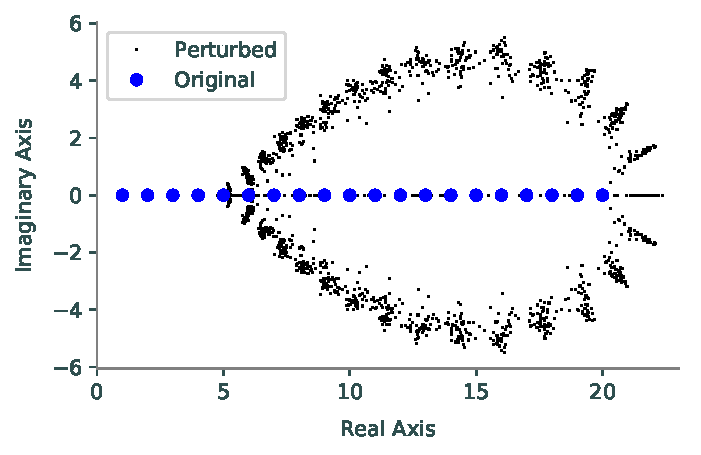
\includegraphics[width=.7\linewidth]{figures/wilkinson_prob_solution.pdf}
\caption{
This figure replicates Figure 12.1 on p. 93 of \emph{Numerical Linear Algebra} by Lloyd N. Trefethen and David Bau III.}
\label{fig:wilkinsonpolynomial_many}
\end{figure}

\label{prob:wilkinson-polynomial-roots}
\label{prob:eigenvalue} % Eigenvalue experiments
Write a function that accepts a matrix $A$ and estimates the condition number of the eigenvalue problem using (\ref{eq:eig-condition-numbers}).
For the perturbation $H$, construct a matrix with complex entries where the real and imaginary parts are drawn from normal distributions centered at $0$ with standard deviation $\sigma = 10^{-10}$.
\begin{lstlisting}
reals = np.random.normal(0, 1e-10, A.shape)
imags = np.random.normal(0, 1e-10, A.shape)
H = reals + 1j*imags
\end{lstlisting}
Use \li{scipy.linalg.eig()} or \li{scipy.linalg.eigvals()} to compute the eigenvalues of $A$ and $A+H$, and use the 2-norm for both the vector and matrix norms.
Return the absolute and relative condition numbers.
\label{prob:eig-condit}

Write a function that accepts bounds $[x_{\min},x_{\max},y_{\min},y_{\max}]$ and an integer \li{res}.
Use your function from Problem \ref{prob:eig-condit} to compute the relative condition number of the eigenvalue problem for the $2\times 2$ matrix
\[
\left[\begin{array}{cc}
1 &  x\\
y & 1\end{array}\right]
\]
at every point of an evenly spaced \li{res}$\times$\li{res} grid over the domain $[x_{\min}, x_{\max}]\times [y_{\min}, y_{\max}]$.
Plot these estimated relative condition numbers using \li{plt.pcolormesh()} and the colormap \li{cmap='gray_r'}.
With \li{res=200}, your plot should look similar to the following figure.

\begin{figure}[H]
    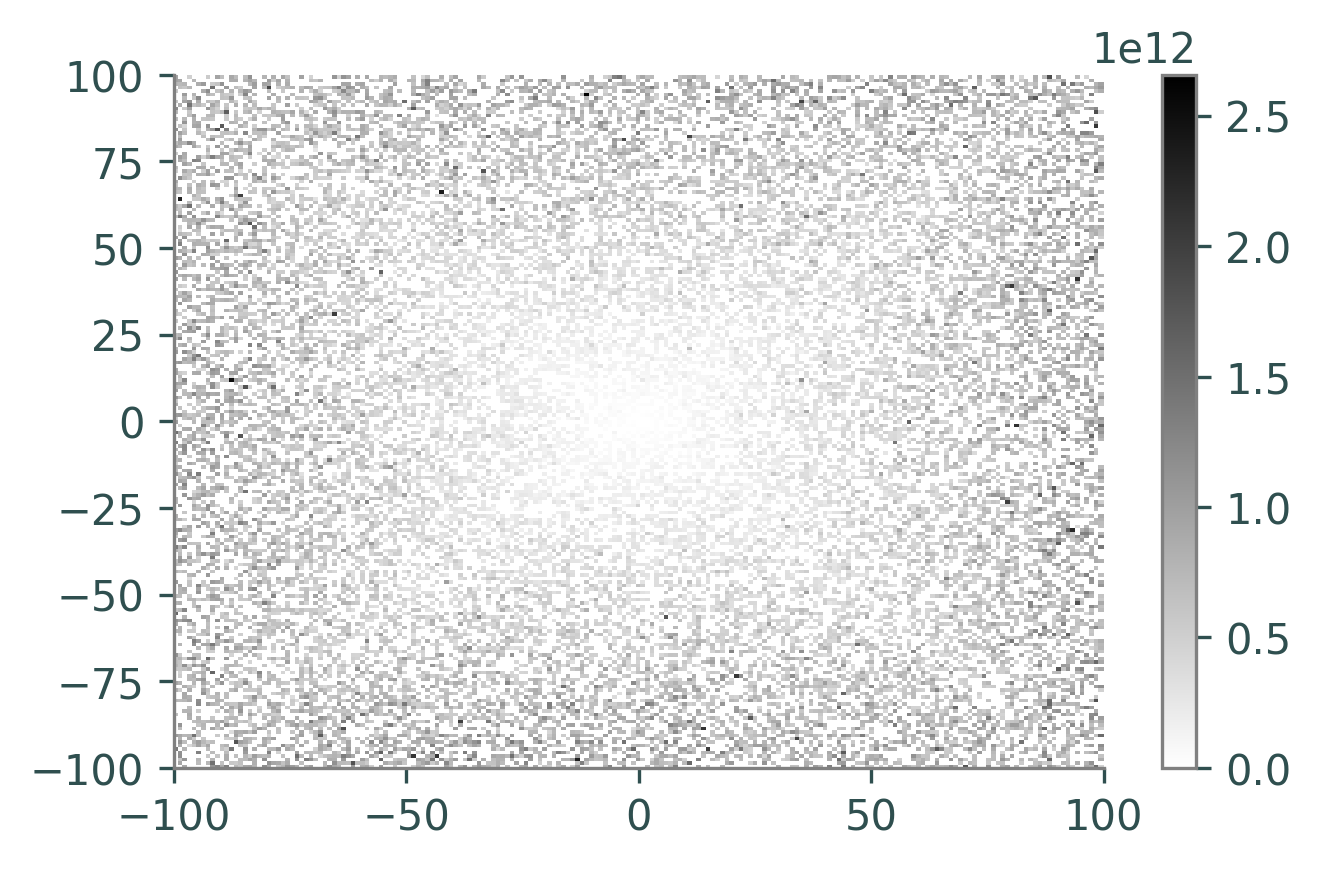
\includegraphics[width=.7\linewidth]{figures/eigenvalue_conditioning.png}
\end{figure}

\label{prob:eigenvalue-conditioning-plot}

Write a function that accepts an integer $n$.
Solve for the coefficients of the polynomial of degree $n$ that best fits the data found in \texttt{stability\_data.npy}.
Use two approaches to get the least squares solution:

\begin{enumerate}
\item Use \li{la.inv()} to solve the normal equations: $\x = (A\trp A)^{-1}A\trp \b$.
Although this approach seems intuitive, it is actually highly unstable and can return an answer with a very large forward error.

\item Use \li{la.qr()} with \li{mode='economic'} and \li{la.solve_triangular()} to solve the system $R\x = Q\trp\b$, which is equivalent to solving the normal equations.
This algorithm has the advantage of being stable.
\end{enumerate}

Load the data and set up the system (\ref{eq:polynomial-least-squares}) with the following code.

\begin{lstlisting}
xk, yk = np.load("stability_data.npy").T
A = np.vander(xk, n+1)
\end{lstlisting}

Plot the resulting polynomials together with the raw data points.
Return the forward error $\norm{A\x-\mathbf{b}}_2$ of both approximations.
\\(Hint: The function \li{np.polyval()} will be helpful for plotting the resulting polynomials.)

Test your function using various values of $n$, taking special note of what happens for values of $n$ near $14$ (pictured below).

\begin{figure}[H]
    \centering
    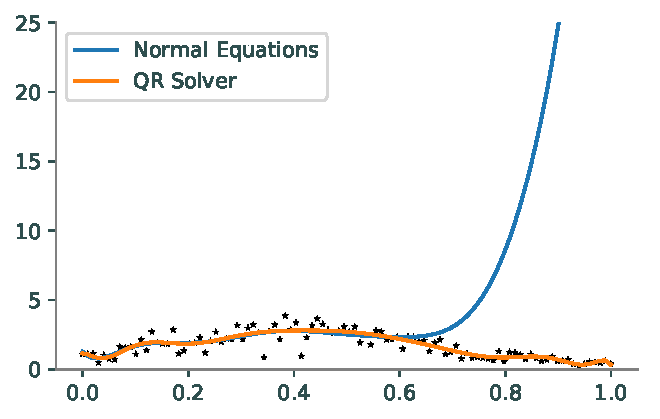
\includegraphics[width=.7\textwidth]{figures/lstsq_stability.pdf}
\end{figure}

Let $I(n) = \int_0^1 x^n e^{x - 1} dx$.
It can be shown that for a positive integer $n$,
\begin{equation}
I(n) = \left(-1\right)^{n} !n + \left(-1\right)^{n + 1} \frac{n!}{e},
\label{eq:integral-subfactorial-formula}
\end{equation}
where $!n=n!\sum_{k=0}^{n} \frac{(-1)^k}{k!}$ is the \emph{subfactorial} of $n$.
Write a function to do the following.
\begin{enumerate}
\item Use SymPy's \li{sy.integrate()} to evaluate the integral form of $I(n)$ for $n=5,10,\ldots,50$.
Convert the symbolic results of each integration to a float.
Since this is done symbolically, these values can be accepted as the true values of $I(n)$.
\\(Hint: be careful that the values of $n$ in the integrand are actual integers, not floats.)

\item Use (\ref{eq:integral-subfactorial-formula}) to compute $I(n)$ for the same values of $n$.
Use \li{sy.subfactorial()} to compute $!n$ and \li{sy.factorial()} to compute $n!$.
\\(Hint: be careful to only pass actual integers to these functions.)
\label{step:subfactorial-cheat}

\item Plot the relative forward error of the results computed in step \ref{step:subfactorial-cheat} at each of the given values of $n$.
Use a log scale on the $y$-axis.
Is (\ref{eq:integral-subfactorial-formula}) a stable way to compute $I(n)$?
Why?
\end{enumerate}
